\documentclass[18pt]{beamer}
\usepackage[utf8]{inputenc} % for the umlauts
\usepackage{subfigure}

\beamertemplatenavigationsymbolsempty
%% SLIDE FORMAT

% use 'beamerthemekit' for standard 4:3 ratio
% for widescreen slides (16:9), use 'beamerthemekitwide'

\usepackage{templates/beamerthemekit}
% \usepackage{templates/beamerthemekitwide}

\setcounter{tocdepth}{1}

%% TITLE PICTURE

% if a custom picture is to be used on the title page, copy it into the 'logos'
% directory, in the line below, replace 'mypicture' with the 
% filename (without extension) and uncomment the following line
% (picture proportions: 63 : 20 for standard, 169 : 40 for wide
% *.eps format if you use latex+dvips+ps2pdf, 
% *.jpg/*.png/*.pdf if you use pdflatex)

%\titleimage{mypicture}

%% TikZ INTEGRATION

% use these packages for PCM symbols and UML classes
% \usepackage{templates/tikzkit}
% \usepackage{templates/tikzuml}

% the presentation starts here

\usepackage{picture}
\usepackage[absolute,overlay]{textpos}
%\usepackage[texcoord,grid,gridunit=mm,gridcolor=red, subgridcolor=green]{eso-pic}
\setbeamercovered{invisible}

\title[SWT1]{Softwaretechnik 1 - 2. Tutorium}
\subtitle{Tutorium 03}
\author{Felix Bachmann}
\date{29.05.2017}

\institute{KIT - Institut für Programmstrukturen und Datenorganisation (IPD)}

% Bibliography

\usepackage[citestyle=authoryear,bibstyle=numeric,hyperref,backend=biber]{biblatex}
\addbibresource{templates/example.bib}
\bibhang1em

\begin{document}

% change the following line to "ngerman" for German style date and logos
\selectlanguage{ngerman}

%title page
\begin{frame}
\titlepage
\end{frame}

\section{Orga}
	\subsection{Feedback 2. Übungsblatt}
	\begin{frame}
		\frametitle{2. Übungsblatt Statistik}
		%TODO add statistics chart [scale=0.7]{./pics/tut2/statistics_ub1.png}
	\end{frame}
	
	\subsection{2. Übungsblatt - Fehler (Allgemein)}
	\begin{frame}
		\frametitle{Häufige Fehler}
		\begin{block}{Allgemein}
			%TODO add common faults
		\end{block}
	\end{frame}
	
	\subsection{2. Übungsblatt - Fehler}
	\begin{frame}
		\frametitle{Häufige Fehler}
		\begin{block}{Aufgabe 1 (??)}
			%TODO add exercise specific faults
		\end{block}
	\end{frame}


\section{Zustandsdiagramm}
	\subsection{Intro(1)}
	\begin{frame}
		\frametitle{Wo sind wir? Pflichtenheft!}
		\begin{enumerate}
			\item Zielbestimmung  
			\item Produkteinsatz 
			\item Produktumgebung
			\item Funktionale Anforderungen 
			\item Produktdaten 
			\item Nichtfunktionale Anforderungen 
			\item Globale Testfälle
			\item Systemmodelle
			\begin{itemize}
				\item Szenarien
				\item Anwendungsfälle
				\item Objektmodelle $\implies$ UML-Klassendiagramme (letztes mal)
				\item \underline{\textbf{Dynamische Modelle}}
				\begin{itemize}
					\item UML-Zustandsdiagramm
					\item UML-Aktivitätsdiagramm
					\item UML-Sequenzdiagramm
					\makebox(0,0){\put(0,3.3\normalbaselineskip){%
							$\left.\rule{0pt}{1.5\normalbaselineskip}\right\}$ Heute!}}
				\end{itemize}
				\item Benutzerschnittstelle$\implies$ Zeichnungen/Screenshots
			\end{itemize}
			\item Glossar 
		\end{enumerate}
	\end{frame}

	\subsection{Intro(2)}
	\begin{frame}
		\frametitle{Begriffsklärung}
		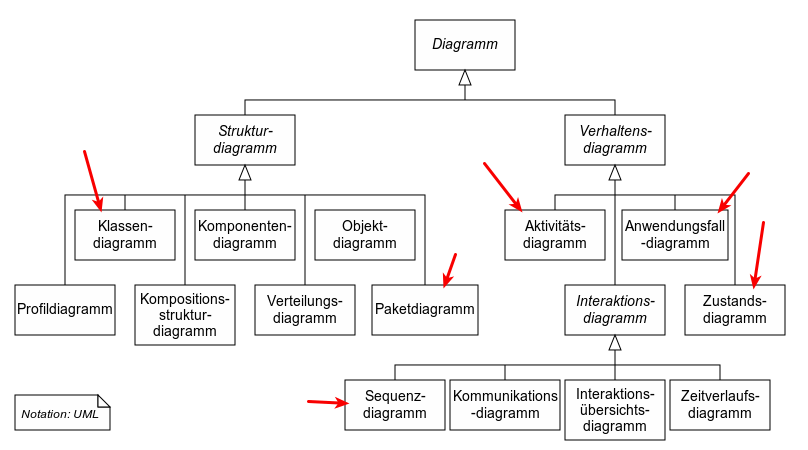
\includegraphics[scale=0.35]{./pics/tut1/uml_diagrams.png}
	\end{frame}

	\subsection{ZD: Allgemein}
	\begin{frame}
		\frametitle{Zustandsdiagramm - Allgemein}
		\begin{block}{Wozu braucht man das?}
			\pause
			\begin{itemize}
				\item Zustand \textbf{eines Objektes} beschreiben
				\item Zustandsüberführungsfunktion?
			\end{itemize}
		\end{block}
	\end{frame}

	\subsection{ZD: Allgemein (2)}
	\begin{frame}
		\frametitle{Zustandsdiagramm $\approx$ endlicher Automat}
					\begin{figure}
			\subfigure[GBI: DEA]{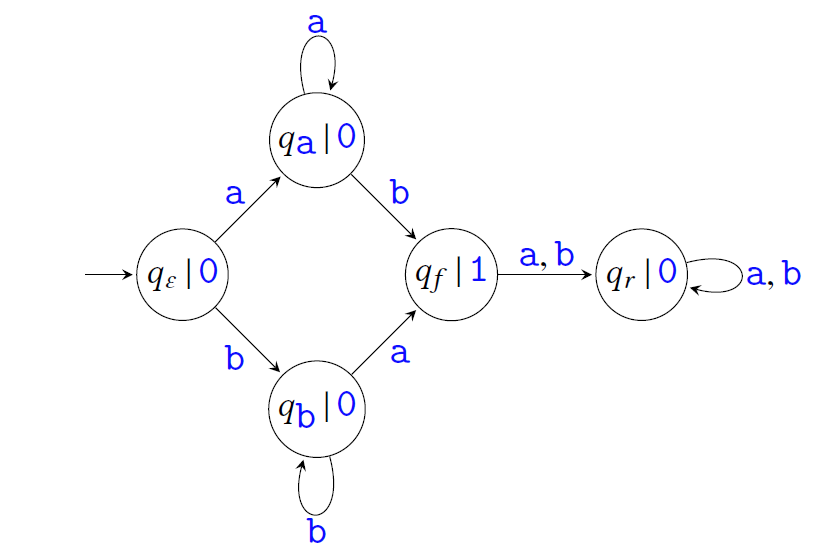
\includegraphics[scale=0.23]{./pics/tut2/auto_gbi.png}}
			\subfigure[SWT: Zustandsdiagramm]{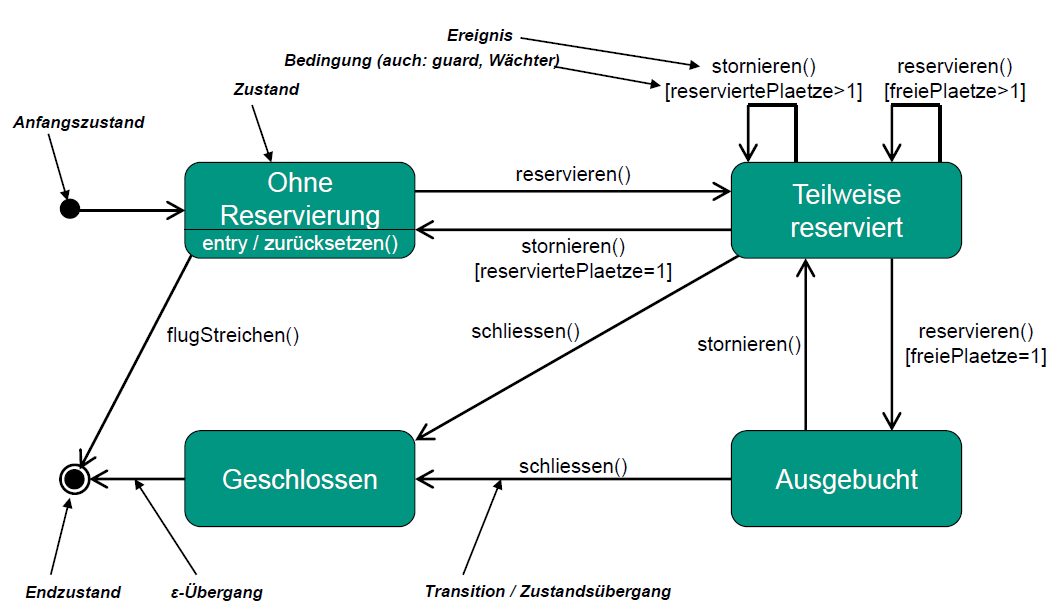
\includegraphics[scale=0.2]{./pics/tut2/auto_swt.png}}
		\end{figure}
	\end{frame}

	\subsection{ZD: Syntax(1)}
	\begin{frame}
		\frametitle{Zustandsdiagramm: Syntax}
		\begin{figure}
			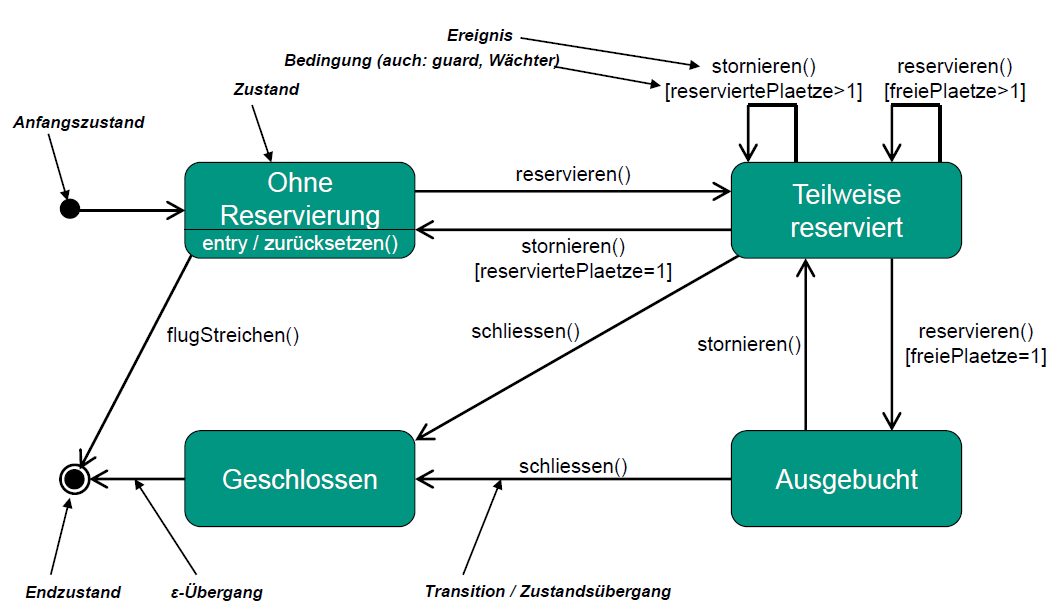
\includegraphics[scale=0.4]{./pics/tut2/auto_swt.png}
		\end{figure}	
	\end{frame}

	\subsection{ZD: Syntax (2)}
	\begin{frame}
		\frametitle{Zustandsdiagramm: Hierarchie}
		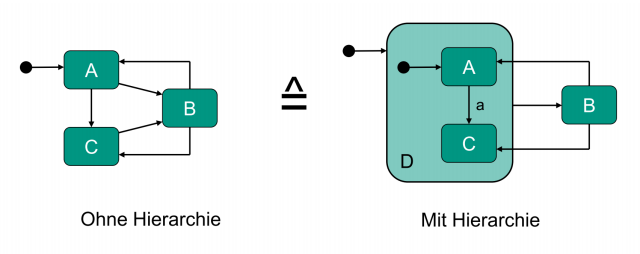
\includegraphics[scale=0.7]{./pics/tut2/auto_hier.png}	
	\end{frame}

	\subsection{ZD: Syntax (3)}
	\begin{frame}
		\frametitle{Zustandsdiagramm: Hierarchie - History}
		\begin{itemize}
			\item  History-Element, damit sich Hierarchie den letzten Zustand merkt
		\end{itemize}
		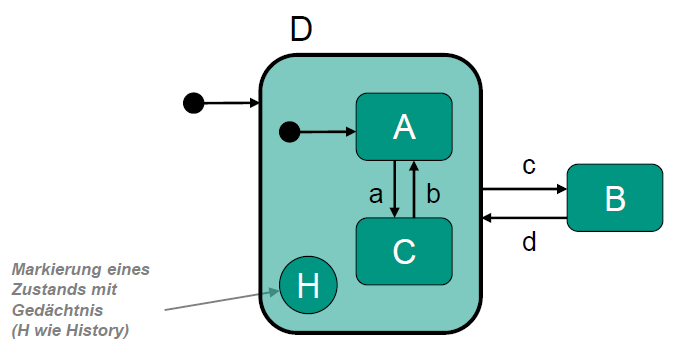
\includegraphics[scale=0.5]{./pics/tut2/auto_hier-hist.png}	
	\end{frame}

	\subsection{ZD: Syntax(4)}
	\begin{frame}
		\frametitle{Zustandsdiagramm: Nebenläufigkeit}	
		\begin{itemize}
			\item  mehrere Zustandsdiagramme in einem
		\end{itemize}
		\centering
		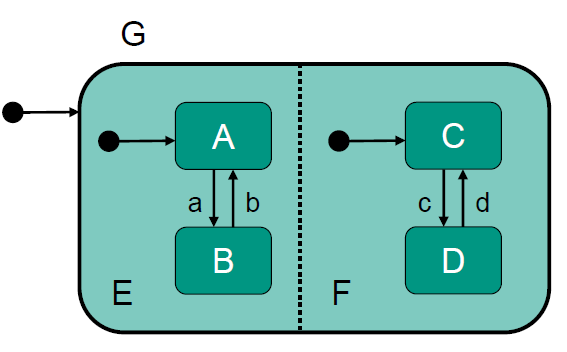
\includegraphics[scale=0.5]{./pics/tut2/auto_par.png}	
	\end{frame}

	\subsection{ZD: Aufgabe}
	\begin{frame}
		\frametitle{Klausuraufgabe SS09}
		Gegeben ist der folgende UML-Zustandsautomat. Geben Sie an, in welcher Zustandskombination
		sich der Zustandsautomat, jeweils ausgehend vom Startzustand, nach den beiden Eingabefolgen
		befindet.
		\centering
		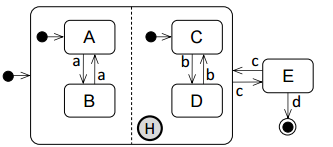
\includegraphics[scale=0.7]{./pics/tut2/auto_ex.png}
		\begin{itemize}
			\item a, b, c, c \pause $\implies$ AxD
			\item c, c, a, b, b, a, c, c, a \pause $\implies$ BxC
		\end{itemize}
	\end{frame}
		
\section{Aktivitätsdiagramm}
	\subsection{AD: Allgemein(1)}
	\begin{frame}
		\frametitle{Aktivitätsdiagramm - Allgemein}
		\begin{block}{Wozu braucht man das?}
			\pause
			\begin{itemize}
				\item Ablaufbeschreibungen (Kontrollfluss, Objektfluss)
				\item i.A. \textbf{mehrere verschiedene} Objekte
			\end{itemize}
		\end{block}
	\end{frame}

	\subsection{AD: Allgemein(2)}
	\begin{frame}
		\frametitle{Aktivitätsdiagramm - Beispiel}
		\begin{itemize}
			\item ist ebenfalls nicht neues!
		\end{itemize}
		\centering
		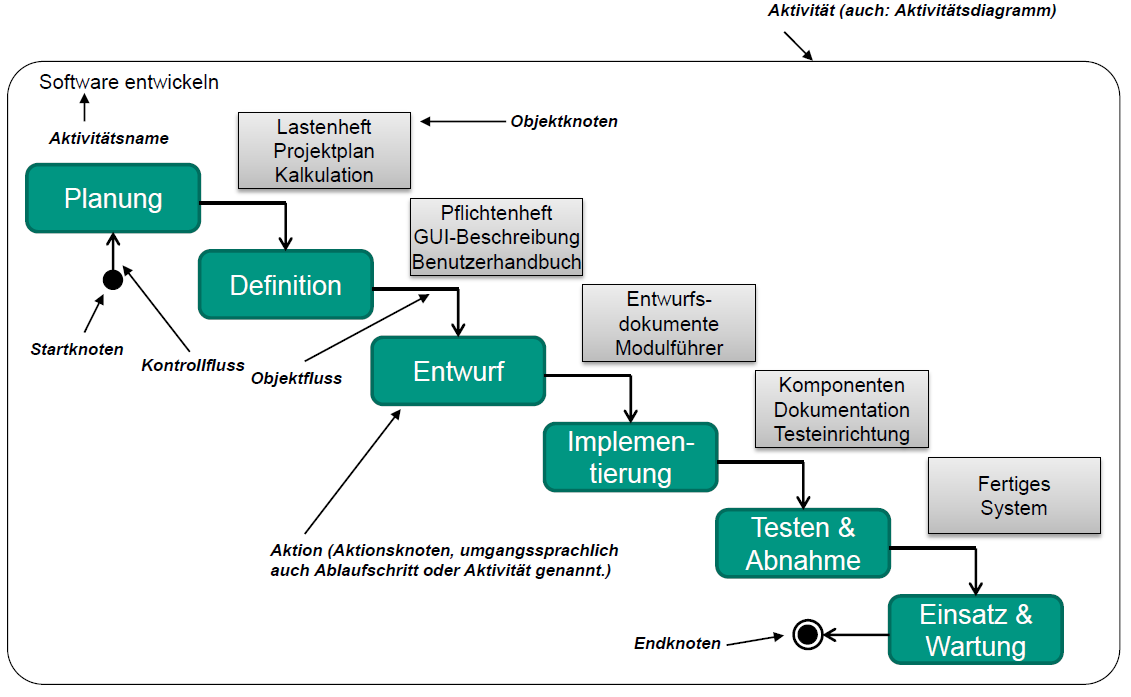
\includegraphics[scale=0.35]{./pics/tut2/act_wat.png}
	\end{frame}

	\subsection{AD: Syntax(1)}
	\begin{frame}
		\frametitle{Aktivitätsdiagramm - Syntax}
		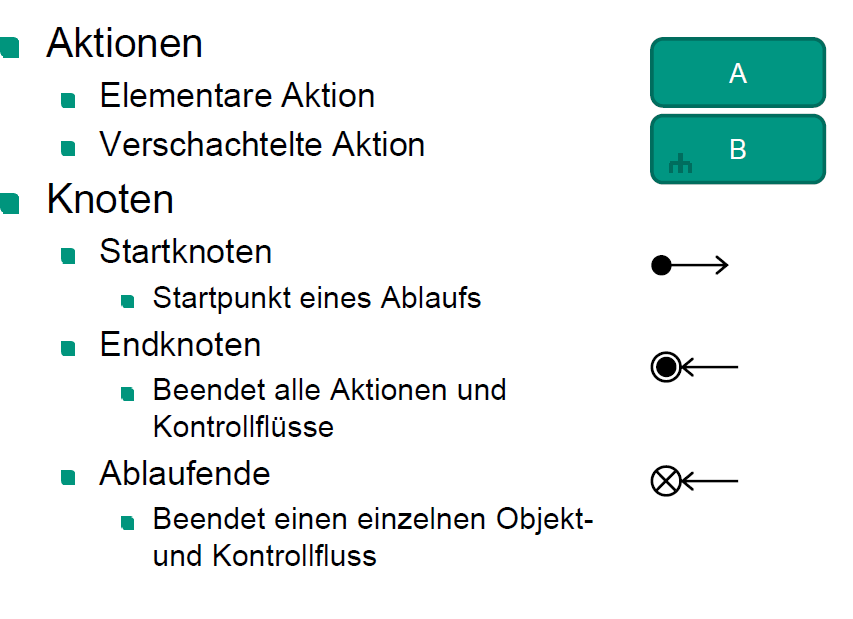
\includegraphics[scale=0.45]{./pics/tut2/act_syn1.png}
	\end{frame}

	\subsection{AD: Syntax(2)}
	\begin{frame}
		\frametitle{Aktivitätsdiagramm - Syntax}
		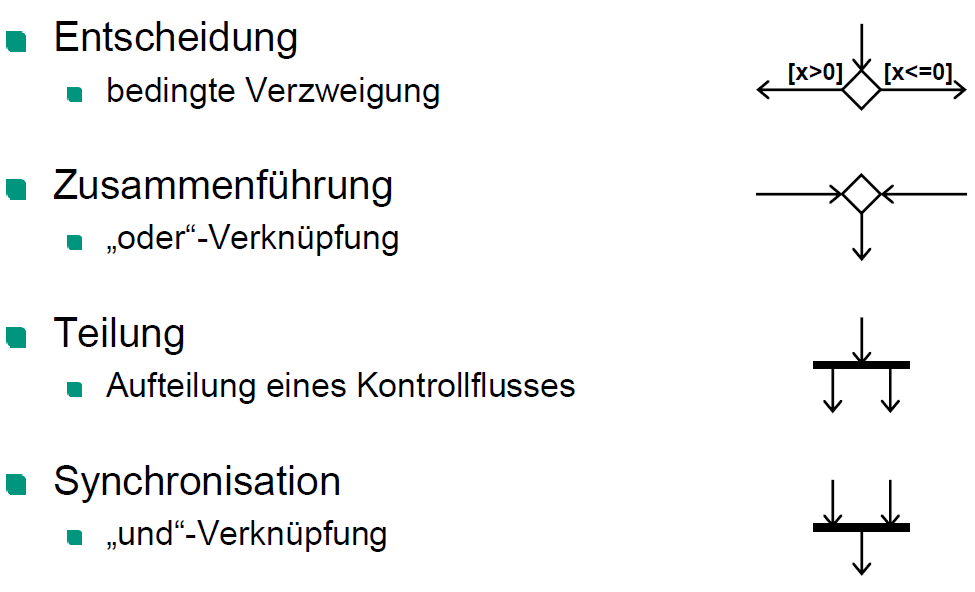
\includegraphics[scale=0.45]{./pics/tut2/act_syn2.png}
	\end{frame}

	\subsection{AD: Syntax(3)}
	\begin{frame}
		\frametitle{Aktivitätsdiagramm - Syntax}
		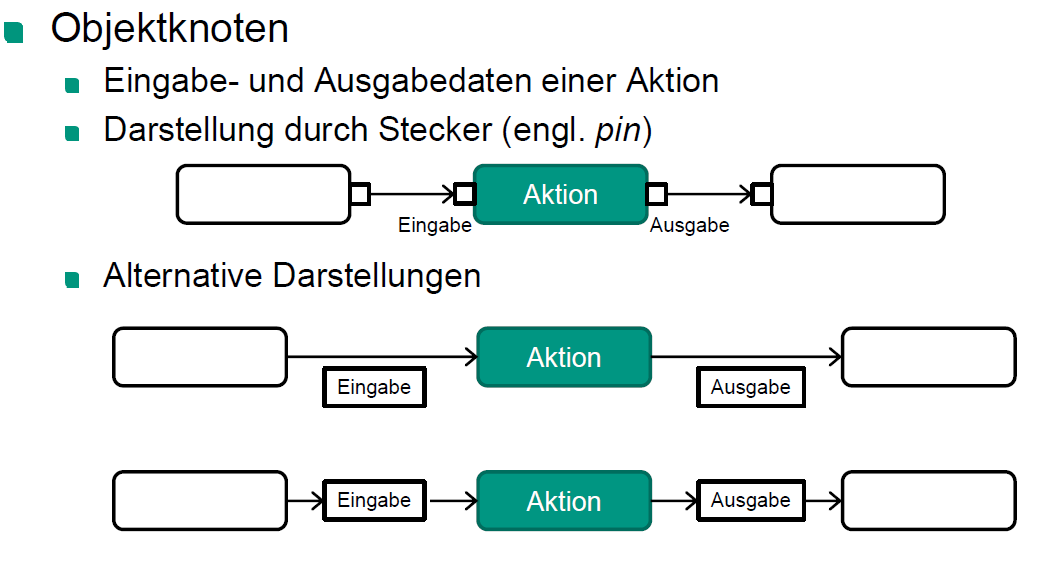
\includegraphics[scale=0.45]{./pics/tut2/act_syn3.png}
	\end{frame}

	\subsection{AD: Ablauf}
	\begin{frame}
		\frametitle{Aktivitätsdiagramm - Ablauf}
		\begin{itemize}
			\item Start am Startknoten mit einer Marke
			\item Aktivitäten werden erst ausgeführt, wenn an jedem Eingang eine Marke anliegt
			\item wurde eine Aktivität ausgeführt, erscheinen an all ihren Ausgängen Marken
		\end{itemize}
	\end{frame}

	\subsection{AD: Beispiel}
	\begin{frame}
		\frametitle{Aktivitätsdiagramm - Beispiel}
		\begin{figure}
			\centering
			\caption{Wie kommt man hier zum Endknoten?}
			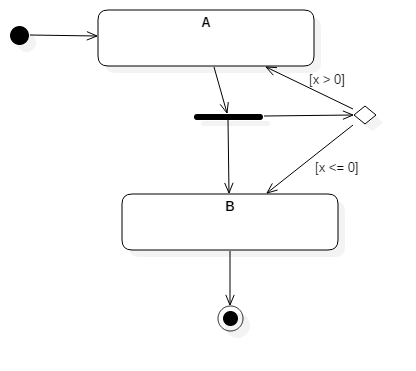
\includegraphics[scale=0.4]{./pics/tut2/act_ex.png}
		\end{figure}
	\end{frame}
		
\section{Tipps}
	\subsection{Tipps}
	\begin{frame}
		\frametitle{Tipps - 3. Übungsblatt}
		\begin{small}
			\begin{exampleblock}{Aufgabe 1-3: Plug-In programmieren}
				\begin{itemize}
					\item l%TODO tipps? allgemein javadoc etc.? [abhängig von UB 2]
				\end{itemize}
			\end{exampleblock}
			\pause
			\begin{exampleblock}{Aufgabe 4: Aktivitätsdiagramm}
				\begin{itemize}
					\item l%TODO tipps
				\end{itemize}
			\end{exampleblock}
			\pause
			\begin{exampleblock}{Aufgabe 5: Sequenzdiagramm}
				\begin{itemize}
					\item l%TODO tipps
				\end{itemize}
			\end{exampleblock}
		\end{small}
	\end{frame}
	
	\subsection{Abgabe}
	\begin{frame}
		\frametitle{Denkt dran!}
		\begin{alertblock}{Abgabe}
			\begin{itemize}
				\item Deadline am 7.6 um 12:00
				\item Aufgabe 4+5 handschriftlich (auf saubere Syntax achten!)
			\end{itemize}
		\end{alertblock}
	\end{frame}
		
	\begin{frame}
		\frametitle{Bis dann! (dann := 12.06.17)}
		\centering
		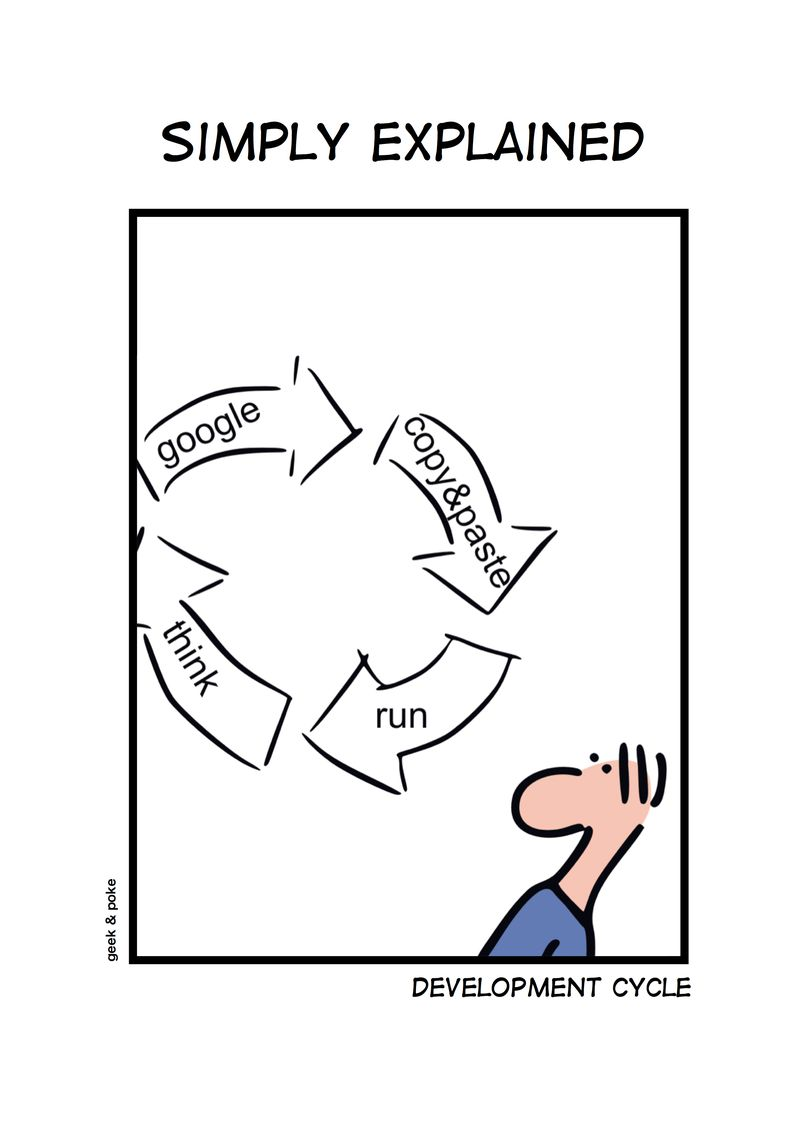
\includegraphics[scale=0.9]{./comics/geek_and_poke_development.jpg}
	\end{frame}

\end{document}
